\begin{blocksection}
\question Would BFS or DFS be better for finding the solution that takes the
least number of moves to solve the game?

\begin{solution}[0.25in]
BFS

Each step in BFS is equivalent to one move, which is the metric we are using.

DFS:
\raisebox{-0.5\height}{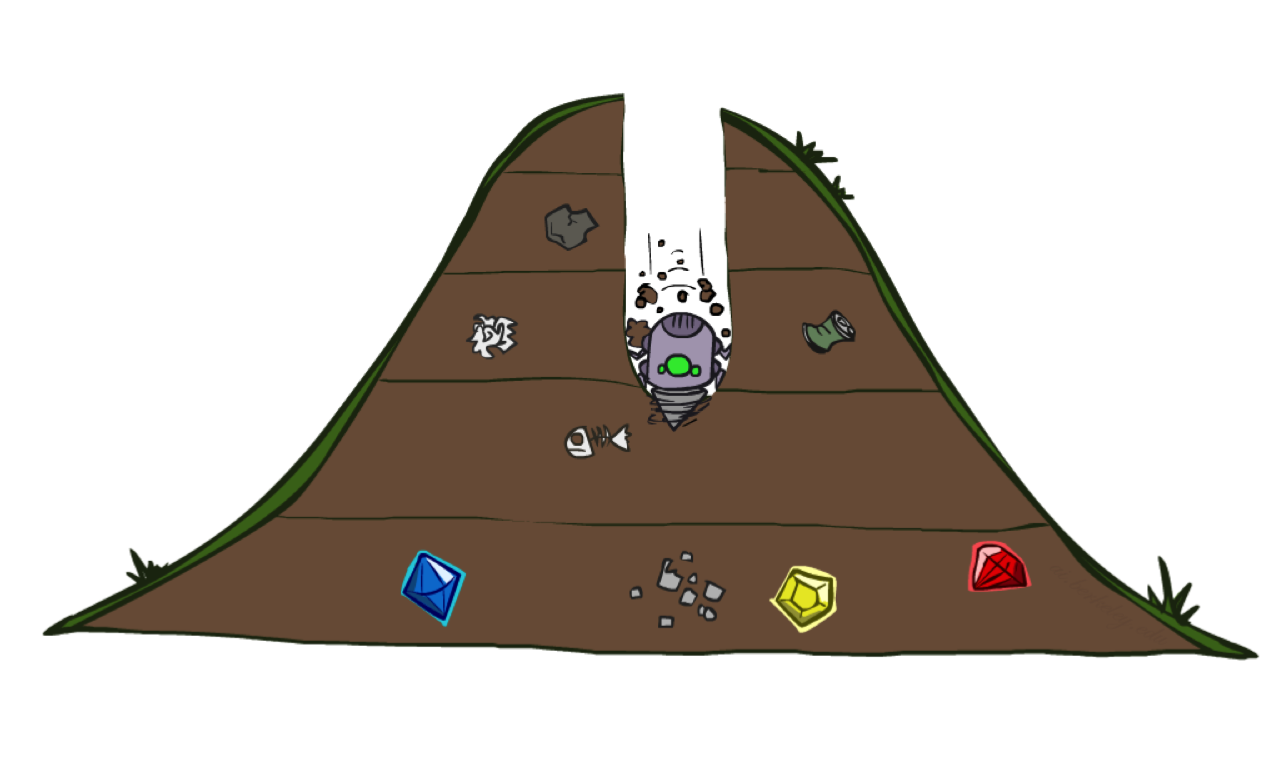
\includegraphics[scale=0.3]{dfs.png}}
\raisebox{-0.5\height}{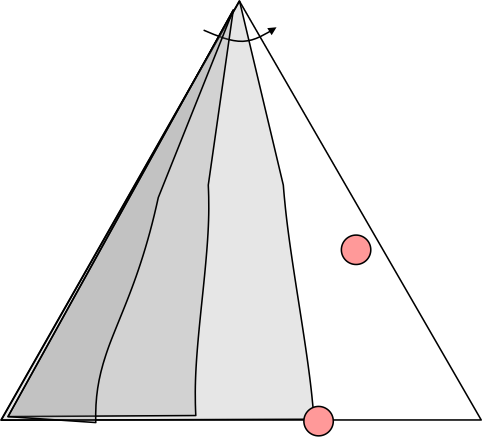
\includegraphics[scale=0.5]{dfs-triangle.png}}

BFS:
\raisebox{-0.5\height}{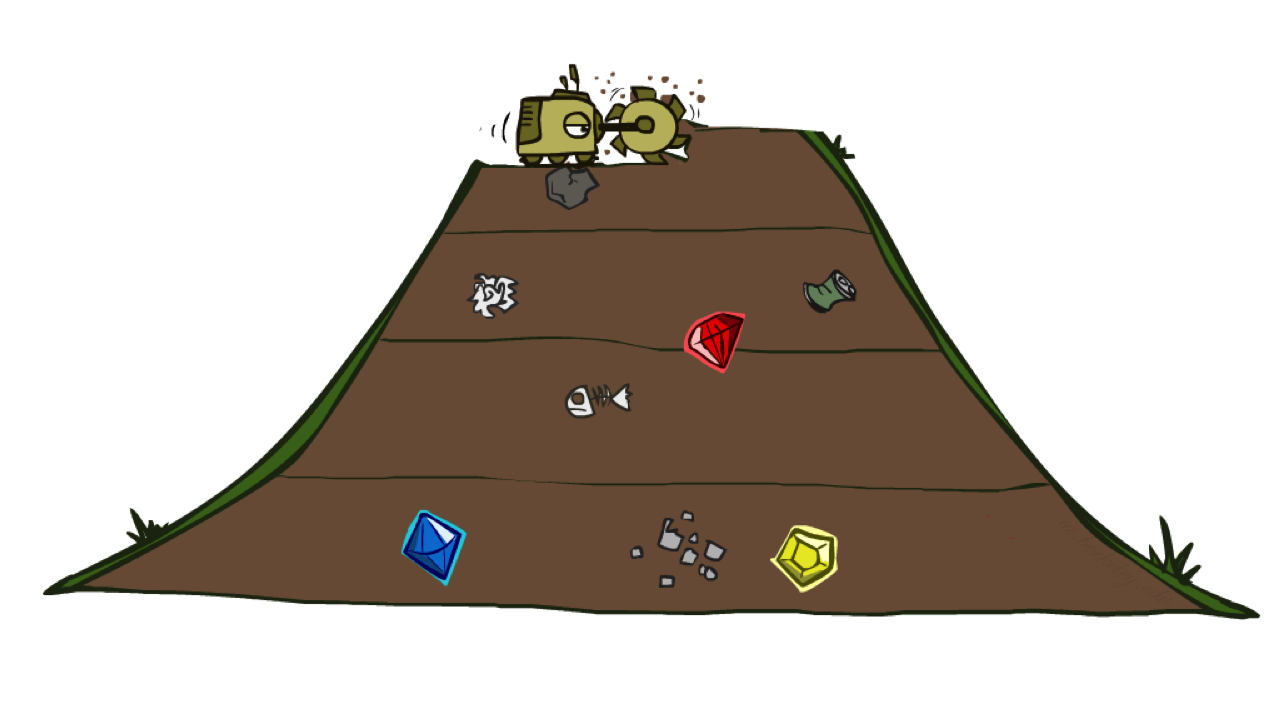
\includegraphics[scale=0.3]{bfs.png}}
\raisebox{-0.5\height}{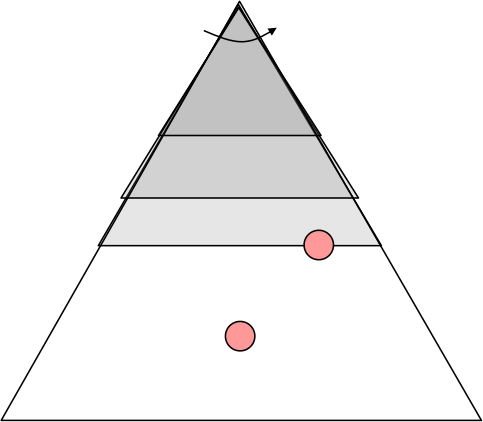
\includegraphics[scale=0.5]{bfs-triangle.png}}

We start the search from the top of the triangle and move downwards. The
circles represent possible solutions.

The first two pictures represent DFS. We see that here, DFS will find the
``leftmost'' solution, even if it is deeper than other solutions. For example,
in the DFS triangle graphic, we see that DFS first finds the bottom left
solution, even though this is more deep (and thus less efficient) than the
solution on the right.

The second two pictures represent BFS.  We see that here, BFS will find the
most optimal solution.  For example, in the BFS triangle graphic, the first
solution returned is the most optimal one (the one closest to the root).

Images from Anca Dragan's CS 188 lecture slides.
\end{solution}
\end{blocksection}
